\chapter{古典密码学}

\section{密码学}

\subsection{密码学(Cryptography)}

密码学是一种用来混淆的技术,它希望将正常的、可识别的信息转变为无法识别的信息。\\

密码学算法可以将明文(plaintext)加密(encrypt)为密文(ciphertext),也可将密文解密(decrypt)为明文。因此密码编码者(cryptographer)需要设计更加安全的加密算法,而破译者(cryptanalyst)的目的就是破解这些加密算法。\\

算法的安全性取决于破解的难度。例如一个旋转密码锁有40个数字,如果密码是一个3元组(如$ 5R, 12L, 7R $),那么可能的密码组合有$ 40^3 = 64000 $种。假设尝试一种组合需要花费10秒,一共需要大约178小时才能尝试完。\\

\begin{figure}[H]
    \centering
    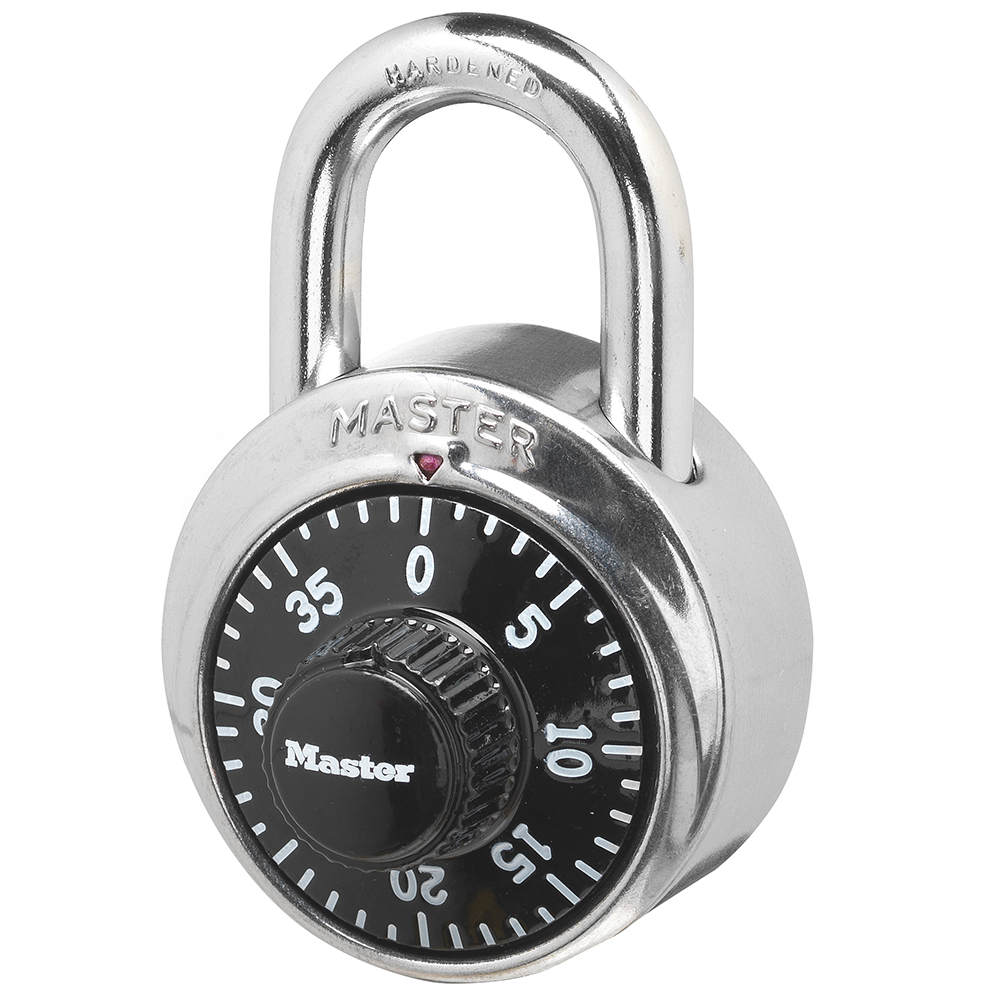
\includegraphics[scale=0.6]{img/C1/1-1/1.png}
    \caption{旋转密码锁}
\end{figure}

如果密码的组合是一个4元组,那么可能的密码组合有$ 40^4 = 2560000 $种。假设尝试一种组合需要花费13秒,一共需要大约9244小时才能尝试完。\\

大部分商业的加密算法是公开的,而军用的加密算法是保密的。\\

\subsection{安全性}

加密算法的安全性分为:

\begin{enumerate}
    \item 无条件安全性(unconditionally secure):即使密码分析者拥有无限的计算资源和密文,都没有足够的信息恢复出明文。事实上,只有一次一密乱码本,才是不可破的,对于实际应用的密码算法都是可破的。在实际中,无条件安全的系统是不存在的。
    \item 计算安全性(Computationally secure):当破解所花费的代价远超于被加密信息的生命周期和本身的价值时,破解就失去了意义。
\end{enumerate}

\newpage

\section{凯撒密码}

\subsection{凯撒密码(Caesar Cipher)}

凯撒密码是一种最简单的加密算法,它是由罗马帝国的凯撒(Julius Caesar)发明的。\\

凯撒加密将明文中的字母用另一个字母来替换,替换的规则是将字母向后移动3位。例如,明文中的A将被替换为D,明文中的B将被替换为E,依此类推。

\begin{itemize}
    \item 明文:meet me after the party
    \item 密文:phhw ph diwhu wkh sduwb
\end{itemize}

破解的方法也很容易,只需要将密文的字母向前移动3位即可。\\

改进后的凯撒加密不再采用固定移动3位的策略,而是可以移动任意位数。对于英文字母的加密而言,一个字母可能被替换为另外的25个字母之一。通过暴力枚举每个移位,还是可以破解凯撒加密。\\

\mybox{凯撒密码(加密)}

\begin{lstlisting}[language=Python]
def encrypt(plaintext, shift=3):
    shift %= 26
    ciphertext = ""

    for c in plaintext:
        if not c.isalpha():
            ciphertext += c
            continue
        if c.isupper():
            ciphertext += chr((ord(c) + shift - 65) % 26 + 65)
        else:
            ciphertext += chr((ord(c) + shift - 97) % 26 + 97)

    return ciphertext
\end{lstlisting}

\vspace{0.5cm}

\mybox{凯撒密码(解密)}

\begin{lstlisting}[language=Python]
def decrypt(ciphertext, shift=3):
    plaintext = ""

    for c in ciphertext:
        if not c.isalpha():
            plaintext += c
            continue
        if c.isupper():
            plaintext += chr((ord(c) - shift - 65) % 26 + 65)
        else:
            plaintext += chr((ord(c) - shift - 97) % 26 + 97)

    return plaintext
\end{lstlisting}

\newpage

\section{单表密码}

\subsection{单表密码(Monoalphabetic Cipher)}

单表密码并不像凯撒密码一样仅仅只是将字母后移,而是随机地将一个字母替换为另一个字母。例如字母的替换规则如下:

\begin{table}[H]
    \centering
    \setlength{\tabcolsep}{1mm}{
        \begin{tabular}{|c|c|c|c|c|c|c|c|c|c|c|c|c|c|c|c|c|c|c|c|c|c|c|c|c|c|}
            \hline
            a & b & c & d & e & f & g & h & i & j & k & l & m & n & o & p & q & r & s & t & u & v & w & x & y & z \\
            \hline
            D & K & V & Q & F & I & B & J & W & P & E & S & C & X & H & T & M & Y & A & U & O & L & R & G & Z & N \\
            \hline
        \end{tabular}
    }
\end{table}

\begin{itemize}
    \item 明文:if we wish to replace letters
    \item 密文:WI RF RWAJ UH YFTSDVF SFUUFYA
\end{itemize}

单表密码一共有$ 25! = 1.55 \times 10^{25} $种可能的替换规则,但是它并不安全。由于人类语言的特性,不同的字母的使用频率是不同的。\\

\begin{figure}[H]
    \centering
    \begin{tikzpicture}
        \scriptsize
        \begin{axis}[width=\linewidth,
                ybar = 1mm,
                bar width = 3mm,
                enlarge x limits=0.04,
                ylabel={Prozentsatz},
                symbolic x coords={a,b,c,d,e,f,g,h,i,j,k,l,m,n,o,p,q,r,s,t,u,v,w,x,y,z},
                xtick=data,
                ymin=0,
                nodes near coords,
                nodes near coords style={rotate=90, anchor=west, font=\footnotesize},
            ]
            \addplot coordinates {
                    (a,8.167)
                    (b,1.492)
                    (c,2.782)
                    (d,4.253)
                    (e,12.702)
                    (f,2.228)
                    (g,2.015)
                    (h,6.094)
                    (i,6.996)
                    (j,0.153)
                    (k,0.772)
                    (l,4.025)
                    (m,2.406)
                    (n,6.749)
                    (o,7.507)
                    (p,1.929)
                    (q,10.095)
                    (r,5.987)
                    (s,6.327)
                    (t,9.056)
                    (u,2.758)
                    (v,0.978)
                    (w,2.360)
                    (x,0.150)
                    (y,1.974)
                    (z,0.074)
                };
        \end{axis}
    \end{tikzpicture}
    \caption{字母使用频率}
\end{figure}

例如有这么一段密文:\\

UZ QSO VUOHXMOPV GPOZPEVSG ZWSZ OPFPESX UDBMETSX

AIZ VUEPHZ HMDZSHZO WSFP APPD TSVP QUZW YMXUZUHSX

EPYEPOPDZSZUFPO MB ZWP FUPZ HMDJ UD TMOHMQ\\

\mybox{字母出现频率}

\begin{lstlisting}[language=Python]
import re

def get_frequency(text):
    frequency = {}
    for c in text:
        if c in frequency:
            frequency[c] += 1
        else:
            frequency[c] = 1
    return frequency


def main():
    with open("ciphertext.txt") as file:
        text = file.readlines()
        text = "".join(text)   
        # remove all non-alphabetic characters
        text = re.sub("[ \n\r]", '', text)

        print(get_frequency(text))


if __name__ == '__main__':
    main()
\end{lstlisting}

这段密文的字母使用频率如下:\\

\{'U': 10, 'Z': 14, 'Q': 3, 'S': 10, 'O': 9, 'V': 5, 'H': 7, 'X': 5, 'M': 8, 'P': 16, 'G': 2, 'E': 6, 'W': 4, 'F': 4, 'D': 6, 'B': 2, 'T': 3, 'A': 2, 'I': 1, 'Y': 2, 'J': 1\}\\

其中P和Z的出现次数最多,分别为16和14次。可以猜测P和Z是对应明文中最常用的字母,因此P和Z非常有可能是e和t。\\

U\textcolor{red}{t} QSO VUOHXMO\textcolor{red}{e}V G\textcolor{red}{e}O\textcolor{red}{t}\textcolor{red}{e}EVSG \textcolor{red}{t}WS\textcolor{red}{t} O\textcolor{red}{e}F\textcolor{red}{e}ESX UDBMETSX

AI\textcolor{red}{t} VUE\textcolor{red}{e}H\textcolor{red}{t} HMD\textcolor{red}{t}SH\textcolor{red}{t}O WSF\textcolor{red}{e} A\textcolor{red}{ee}D TSV\textcolor{red}{e} QU\textcolor{red}{t}W YMXU\textcolor{red}{t}UHSX

E\textcolor{red}{e}YE\textcolor{red}{e}O\textcolor{red}{e}D\textcolor{red}{t}S\textcolor{red}{t}UF\textcolor{red}{e}O MB \textcolor{red}{t}W\textcolor{red}{e} FU\textcolor{red}{et} HMDJ UD TMOHMQ\\

通过英语中单词的组合,可以猜测S对应a、W对应h,因此ZWSZ对应that、ZWP对应the。\\

U\textcolor{red}{t} Q\textcolor{red}{a}O VUOHXMO\textcolor{red}{e}V G\textcolor{red}{e}O\textcolor{red}{t}\textcolor{red}{e}EV\textcolor{red}{a}G \textcolor{red}{that} O\textcolor{red}{e}F\textcolor{red}{e}E\textcolor{red}{a}X UDBMET\textcolor{red}{a}X

AI\textcolor{red}{t} VUE\textcolor{red}{e}H\textcolor{red}{t} HMD\textcolor{red}{ta}H\textcolor{red}{t}O \textcolor{red}{ha}F\textcolor{red}{e} A\textcolor{red}{ee}D T\textcolor{red}{a}V\textcolor{red}{e} QU\textcolor{red}{th} YMXU\textcolor{red}{t}UH\textcolor{red}{a}X

E\textcolor{red}{e}YE\textcolor{red}{e}O\textcolor{red}{e}D\textcolor{red}{ta}\textcolor{red}{t}UF\textcolor{red}{e}O MB \textcolor{red}{the} FU\textcolor{red}{et} HMDJ UD TMOHMQ\\

依次类推,可以破解整个密文:\\

it was disclosed yesterday that several informal

but direct contacts have been made with political

representatives of the viet cong in moscow

\newpage

\section{维吉尼亚密码}

\subsection{维吉尼亚密码(Vigenere Cipher)}

维吉尼亚密码是在凯撒密码的基础上产生的一种加密方法,它将凯撒密码的全部25种位移排序为一张表,与原字母序列共同组成26行26列的密码表。\\

\begin{table}[H]
    \centering
    \setlength{\tabcolsep}{0.5mm}{
        \begin{tabular}{c|c|c|c|c|c|c|c|c|c|c|c|c|c|c|c|c|c|c|c|c|c|c|c|c|c|c|}
                       & \textbf{A} & \textbf{B} & \textbf{C} & \textbf{D} & \textbf{E} & \textbf{F} & \textbf{G} & \textbf{H} & \textbf{I} & \textbf{J} & \textbf{K} & \textbf{L} & \textbf{M} & \textbf{N} & \textbf{O} & \textbf{P} & \textbf{Q} & \textbf{R} & \textbf{S} & \textbf{T} & \textbf{U} & \textbf{V} & \textbf{W} & \textbf{X} & \textbf{Y} & \textbf{Z} \\
            \hline
            \textbf{A} & A          & B          & C          & D          & E          & F          & G          & H          & I          & J          & K          & L          & M          & N          & O          & P          & Q          & R          & S          & T          & U          & V          & W          & X          & Y          & Z          \\[-1ex]
            \hline
            \textbf{B} & B          & C          & D          & E          & F          & G          & H          & I          & J          & K          & L          & M          & N          & O          & P          & Q          & R          & S          & T          & U          & V          & W          & X          & Y          & Z          & A          \\[-1ex]
            \hline
            \textbf{C} & C          & D          & E          & F          & G          & H          & I          & J          & K          & L          & M          & N          & O          & P          & Q          & R          & S          & T          & U          & V          & W          & X          & Y          & Z          & A          & B          \\[-1ex]
            \hline
            \textbf{D} & D          & E          & F          & G          & H          & I          & J          & K          & L          & M          & N          & O          & P          & Q          & R          & S          & T          & U          & V          & W          & X          & Y          & Z          & A          & B          & C          \\[-1ex]
            \hline
            \textbf{E} & E          & F          & G          & H          & I          & J          & K          & L          & M          & N          & O          & P          & Q          & R          & S          & T          & U          & V          & W          & X          & Y          & Z          & A          & B          & C          & D          \\[-1ex]
            \hline
            \textbf{F} & F          & G          & H          & I          & J          & K          & L          & M          & N          & O          & P          & Q          & R          & S          & T          & U          & V          & W          & X          & Y          & Z          & A          & B          & C          & D          & E          \\[-1ex]
            \hline
            \textbf{G} & G          & H          & I          & J          & K          & L          & M          & N          & O          & P          & Q          & R          & S          & T          & U          & V          & W          & X          & Y          & Z          & A          & B          & C          & D          & E          & F          \\[-1ex]
            \hline
            \textbf{H} & H          & I          & J          & K          & L          & M          & N          & O          & P          & Q          & R          & S          & T          & U          & V          & W          & X          & Y          & Z          & A          & B          & C          & D          & E          & F          & G          \\[-1ex]
            \hline
            \textbf{I} & I          & J          & K          & L          & M          & N          & O          & P          & Q          & R          & S          & T          & U          & V          & W          & X          & Y          & Z          & A          & B          & C          & D          & E          & F          & G          & H          \\[-1ex]
            \hline
            \textbf{J} & J          & K          & L          & M          & N          & O          & P          & Q          & R          & S          & T          & U          & V          & W          & X          & Y          & Z          & A          & B          & C          & D          & E          & F          & G          & H          & I          \\[-1ex]
            \hline
            \textbf{K} & K          & L          & M          & N          & O          & P          & Q          & R          & S          & T          & U          & V          & W          & X          & Y          & Z          & A          & B          & C          & D          & E          & F          & G          & H          & I          & J          \\[-1ex]
            \hline
            \textbf{L} & L          & M          & N          & O          & P          & Q          & R          & S          & T          & U          & V          & W          & X          & Y          & Z          & A          & B          & C          & D          & E          & F          & G          & H          & I          & J          & K          \\[-1ex]
            \hline
            \textbf{M} & M          & N          & O          & P          & Q          & R          & S          & T          & U          & V          & W          & X          & Y          & Z          & A          & B          & C          & D          & E          & F          & G          & H          & I          & J          & K          & L          \\[-1ex]
            \hline
            \textbf{N} & N          & O          & P          & Q          & R          & S          & T          & U          & V          & W          & X          & Y          & Z          & A          & B          & C          & D          & E          & F          & G          & H          & I          & J          & K          & L          & M          \\[-1ex]
            \hline
            \textbf{O} & O          & P          & Q          & R          & S          & T          & U          & V          & W          & X          & Y          & Z          & A          & B          & C          & D          & E          & F          & G          & H          & I          & J          & K          & L          & M          & N          \\[-1ex]
            \hline
            \textbf{P} & P          & Q          & R          & S          & T          & U          & V          & W          & X          & Y          & Z          & A          & B          & C          & D          & E          & F          & G          & H          & I          & J          & K          & L          & M          & N          & O          \\[-1ex]
            \hline
            \textbf{Q} & Q          & R          & S          & T          & U          & V          & W          & X          & Y          & Z          & A          & B          & C          & D          & E          & F          & G          & H          & I          & J          & K          & L          & M          & N          & O          & P          \\[-1ex]
            \hline
            \textbf{R} & R          & S          & T          & U          & V          & W          & X          & Y          & Z          & A          & B          & C          & D          & E          & F          & G          & H          & I          & J          & K          & L          & M          & N          & O          & P          & Q          \\[-1ex]
            \hline
            \textbf{S} & S          & T          & U          & V          & W          & X          & Y          & Z          & A          & B          & C          & D          & E          & F          & G          & H          & I          & J          & K          & L          & M          & N          & O          & P          & Q          & R          \\[-1ex]
            \hline
            \textbf{T} & T          & U          & V          & W          & X          & Y          & Z          & A          & B          & C          & D          & E          & F          & G          & H          & I          & J          & K          & L          & M          & N          & O          & P          & Q          & R          & S          \\[-1ex]
            \hline
            \textbf{U} & U          & V          & W          & X          & Y          & Z          & A          & B          & C          & D          & E          & F          & G          & H          & I          & J          & K          & L          & M          & N          & O          & P          & Q          & R          & S          & T          \\[-1ex]
            \hline
            \textbf{V} & V          & W          & X          & Y          & Z          & A          & B          & C          & D          & E          & F          & G          & H          & I          & J          & K          & L          & M          & N          & O          & P          & Q          & R          & S          & T          & U          \\[-1ex]
            \hline
            \textbf{W} & W          & X          & Y          & Z          & A          & B          & C          & D          & E          & F          & G          & H          & I          & J          & K          & L          & M          & N          & O          & P          & Q          & R          & S          & T          & U          & V          \\[-1ex]
            \hline
            \textbf{X} & X          & Y          & Z          & A          & B          & C          & D          & E          & F          & G          & H          & I          & J          & K          & L          & M          & N          & O          & P          & Q          & R          & S          & T          & U          & V          & W          \\[-1ex]
            \hline
            \textbf{Y} & Y          & Z          & A          & B          & C          & D          & E          & F          & G          & H          & I          & J          & K          & L          & M          & N          & O          & P          & Q          & R          & S          & T          & U          & V          & W          & X          \\[-1ex]
            \hline
            \textbf{Z} & Z          & A          & B          & C          & D          & E          & F          & G          & H          & I          & J          & K          & L          & M          & N          & O          & P          & Q          & R          & S          & T          & U          & V          & W          & X          & Y          \\[-1ex]
            \hline
        \end{tabular}
    }
    \caption{维吉尼亚密码表}
\end{table}

除了密码表,还必须有一个密钥(key)。密钥由字母组成,最少一个字母,最多可与明文字母数相等。如果密钥只有1个字母,相当于凯撒密码。\\

\subsection{加密}

例如:

\begin{itemize}
    \item 明文:I Love You
    \item 密钥:OK
\end{itemize}

首先,如果密钥长度小于明文长度(非字母忽略),就重复拼接密钥,使其与明文长度相等。

\begin{itemize}
    \item 明文:I Love You
    \item 密钥:OKOKOKOK
\end{itemize}

接着根据密码表进行加密。明文第一个字母是I,密钥的第一个字母是O,因此在查找密码表的I行O列,得到加密后的字母W。同理,第二个字母为位于L行K列的字母V。\\

依次类推,得到密文:W VCFS ICE。\\

\subsection{解密}

例如:

\begin{itemize}
    \item 密文:PWZRNZBZEANQKBUHNLNB
    \item 密钥:WIND
\end{itemize}

首先把密钥重复拼接,直到和密文长度相同。

\begin{itemize}
    \item 密文:PWZRNZBZEANQKBUHNLNB
    \item 密钥:WINDWINDWINDWINDWIND
\end{itemize}

根据密文的第一个字母P,在密码表中找到P行,在P行找出值为W的列,沿着该列向上找到该列为T,因此P解密后可以得到T。\\

根据相同的方法,可以得到明文:TOMORROWISANOTHERDAY。\\

\mybox{维吉尼亚密码}

\begin{lstlisting}[language=Python]
import re

def generate_key(plaintext, key):
    n = len(plaintext) - len(key)
    for i in range(n): 
        key += key[i % len(key)]
    return key


def encrypt(plaintext, key):
    # remove all non-alphabetic characters
    plaintext = re.sub("[ \n\r]", '', plaintext).upper()
    key = generate_key(plaintext, key)

    ciphertext = ""
    for i in range(len(plaintext)):
        ciphertext += chr((ord(plaintext[i]) + ord(key[i])) % 26 + 65)
    return ciphertext


def decrypt(ciphertext, key):
    # remove all non-alphabetic characters
    ciphertext = re.sub("[ \n\r]", '', ciphertext).upper()
    key = generate_key(ciphertext, key)

    plaintext = ""
    for i in range(len(ciphertext)):
        plaintext += chr((ord(ciphertext[i]) - ord(key[i])) % 26 + 65)
    return plaintext
\end{lstlisting}

\newpage

\section{一次性密码本}

\subsection{一次性密码本(One-Time Pad)}

一次性密码本算法所用的密钥是一次性的,因此不会出现因为密钥泄露导致之前的加密内容被破解的情况。即使密钥被泄露了,也只会影响一次通信过程。\\

计算机在传输数据时,会将文字转换为对应的二进制编码。通过随机生成一个与明文的二进制编码长度相同的密钥,一次性密码本将明文和密钥进行异或(XOR)运算,得到密文。\\

由于XOR运算的特性,即比特位相同为0,不同为1:

\begin{itemize}
    \item 0 XOR 0 = 0
    \item 0 XOR 1 = 1
    \item 1 XOR 0 = 1
    \item 1 XOR 1 = 0
\end{itemize}

同时另一个XOR的特性就是可逆性,即A XOR B = C,则C XOR B = A。那么通过将密文和密钥再次异或操作就可以得到原文。\\

\subsection{优势}

虽然一次性密码本非常简单,但是一次性密码本是无法破译的,这个破译并不是指现有的计算能力不够,而是指即使拥有无穷大的计算能力也无法破译。\\

假如你拿到了一段128 bits的密文,通过遍历等长的密钥进行暴力破解,将会生成$ 2^{128} $个原文,即原文的所有排列组合。\\

在这些排列组合中,可能会出现一些有意义的文字,但是你并不能确定这些文字是否就是原文,因为在所有的排列组合中会产生大量有意义的问题。\\

因此破解一次性密码本算法是无意义的,就像是知道了原文的长度,然后自己构造了一个这个长度的原文。\\

\subsection{缺陷}

既然一次性密码本这么好,那么为什么我们在实际中很少用到呢?

\begin{itemize}
    \item 密钥太长:密钥的长度与原文相同,如果原文很大,那么对应的密钥也很大。

    \item 密钥无法重用:每个密钥只用一次,既是优点也是缺点。这意味着每次都要不停地更换密钥,增加了复杂性。

    \item 密钥的配送:目标端如果想解密就必须拿到密钥,如果能够机密地传输密钥给目标端,那为什么不直接将原文机密地传送给目标端呢?

    \item 密钥的保存:每一个明文都需要保存一个同样长度的密钥。
\end{itemize}

\newpage